\documentclass{beamer}
\usepackage{graphicx}

\setbeamertemplate{footline}[frame number]

\begin{document}
\title{Array-Based Distributed Modifiable Mesh Structure}
\author{Dan Ibanez}

\frame{\titlepage}

\frame{\frametitle{Motivation}
\begin{itemize}
\item Memory per core is decreasing
\item Desired meshes are increasing in element count
\item Flexible workflows when memory use is well below the limit
\item Array storage improves performance
\begin{itemize}
\item Locality of access, cache-friendly
\item Faster I/O
\item Fewer memory allocation calls, allocator fragmentation
\end{itemize}
\item Parallel efficiency and scaling also critical
\end{itemize}
}

\frame{\frametitle{Overview}
\begin{itemize}
\item
We present a mesh data structure with novel properties:
\begin{enumerate}
\item composed of several large arrays
\item addition and removal are $O(1)$ operations
\item supports mixed element types
\item stores arbitrary associated data
\item Reduced form uses up to 10x less memory than full object-based versions
\item efficiently and scalably supports parallel meshes
\end{enumerate}
\end{itemize}
}

\frame{\frametitle{Background: Adjacency Graph}
\begin{itemize}
\item
Element to node connectivity forms a bipartite graph
where all elements of the same topological type
have the same degree.

\item
In this example, both elements are quadrilaterals.

\begin{center}
\includegraphics[width=0.3\textwidth]{ibanez_cse15-1.png}
\hspace{30pt}
\includegraphics[width=0.4\textwidth]{ibanez_cse15-3.png}
\end{center}

\item
At right is the adjacency graph: mesh entities become
graph nodes and adjacency becomes undirected graph edges.
\end{itemize}
}

\frame{\frametitle{New Structure, Part 1: Downward Adjacency}
\begin{itemize}
\item
The simplest mesh data structure is an element to
node connectivity array.

\item
Given an integer element id, returns the integer
node ids of that element.

\item
Sufficient for element integration, element
stiffness matrix assembly, etc.

\begin{center}
\includegraphics[width=0.4\textwidth]{ibanez_cse15-2.png}
\end{center}
\end{itemize}
}

\frame{\frametitle{(Old Structure) Upward Adjacency}
\begin{itemize}
\item
The inverse of element to node connectivity, i.e.
which elements are adjacent to a given node.
This is harder, because the degrees are not the same.

\item
Object-based structures may store many small arrays:

\begin{center}
\includegraphics[width=0.4\textwidth]{ibanez_cse15-4.png}
\end{center}

\item
Uses include:
\begin{itemize}
\item During edge split, get adjacent elements to split
\item Check for mesh entity existence based on its vertices
(used to prevent invalid modification)
\item Element-to-element traversal: get elements around
a starting point (error estimators, particle motion)
\end{itemize}
\end{itemize}
}

\frame{\frametitle{New Structure, Part 2: Linked Upward Adjacency}
\begin{itemize}
\item
We developed a compact yet flexible structure of 2 arrays
\item
The entries of the ``next" array are arranged
to match the ordering of the downward array, such
that the same adjacency graph edge has the same index.
\item
The entries of the ``first" array are accessed by vertex index

\begin{center}
\includegraphics[width=0.45\textwidth]{ibanez_cse15-6.png}
\end{center}

\item
Graph edges from the same graph node are linked together.
Iterating over these links, element index is known
implicitly based on the graph edge index.
\end{itemize}
}

\frame{\frametitle{Modification, Part 1: Entity Addition}
\begin{itemize}
\item
Users create new entities, either by migrating from
another part or mesh refinement.
\item
We implement the common solution of geometric growth
with additions to the end.
\item
Array has allocated capacity $(c)$ and used size.
When addition is requested and used size equals capacity,
reallocate to capacity $\alpha c$, $\alpha > 1$.
We use $\frac32(c+1)$.
\item
Result is amortized $O(1)$ insertion at the end,
\item
Applies to all arrays storing data for that mesh entity type
\end{itemize}
\begin{center}
\includegraphics[width=0.4\textwidth]{ibanez_cse15-9.png}
\end{center}
}

\frame{\frametitle{Modification, Part 2: Entity Removal}
\begin{itemize}
\item
Any entity may be removed by the user, which
removes an entry from each array, leaving a hole in each array.
\item
Trying to fill the hole requires moving another
entry or entries,
but changing indices is bad for users: they
need unique consistent identifiers
\item
So, keep the holes and track them.
Holes are linked together in one ``free list"
array per entity type, which tracks the holes
in all the arrays for that entity type.
\item
Most workflows tend to increase entity counts.
Otherwise, a reordering is needed to move all
holes to the end so their memory can be released.
\end{itemize}
}

\frame{\frametitle{New Structure, Part 3: Entity Add/Remove Summary}
\begin{itemize}
\item
On removal, link new hole into free list.

\item
On addition:
\begin{enumerate}
\item
If there are holes, unlink the first hole
and return its index
\item
If used size equals capacity, reallocate for
bigger capacity
\item
Increment used size, return last index
\end{enumerate}

\vspace{20pt}

\includegraphics[width=0.8\textwidth]{flex.png}
\end{itemize}
}

\frame{\frametitle{Background: Parallel Vertex Remotes}
\begin{itemize}
\item
Copies of the same vertex on different parts are
connected by ``remote entities", or ``remotes".
Example: one vertex, three parts, all neighbors.
\begin{center}
\includegraphics[width=0.7\textwidth]{remotes.png}
\end{center}
\item
Remotes of of the same vertex on the same part
are linked together.
Pairs of remotes on different parts are linked
by ``parallel pointers": (part id, index) tuples.
\end{itemize}
}

\frame{\frametitle{New Structure, Part 4: Remote Arrays}
\begin{itemize}
\item
Remotes are grouped into arrays based on
which neighbor they are linking with:
one array per neighbor.
\begin{center}
\includegraphics[width=0.6\textwidth]{remote_arrays.png}
\end{center}

\item
Another array maps vertices to their
first remote.

\item Each entry in the remote arrays has a parallel
pointer and a normal pointer to the next local remote.
\end{itemize}
}

\frame{\frametitle{New Structure Summary}

\begin{itemize}
\item
A reduced mesh representation with only elements
and vertices would use the following set of arrays:
\begin{enumerate}
\item Vertex free list array
\item Element free list array
\item Element to vertex array
\item Vertex to element lists-in-arrays
\item Vertex remotes
\item Simulation field arrays, indexed by vertex id
\end{enumerate}

\end{itemize}
}

\frame{\frametitle{Memory Analysis}
\begin{itemize}
\item This analysis considers a single part with no remotes
\item Theoretical memory use for a reduced tetrahedral mesh:
\item Static pointers =
$(4+4)n_{tet} + (3)n_{vtx}$
\item With free list =
$(1+4+4)n_{tet} + (1+3)n_{vtx}$
\item Estimated ratios
\[n_{vtx} = n_{tet}/6\]
\item With free list, 56 pointers per vertex, ~9.7 pointers per element
\item Using 32-bit index ``pointers", ~40 bytes per element
\item With non-topological data added, uses ~50 bytes
per element
\end{itemize}
}

\frame{\frametitle{Test 1: Memory Use Comparison}
\begin{itemize}
\item
We compare the total memory use of various codes for
storing connectivity and coordinates of a 100K tetrahedron
mesh on a single part.
\begin{center}
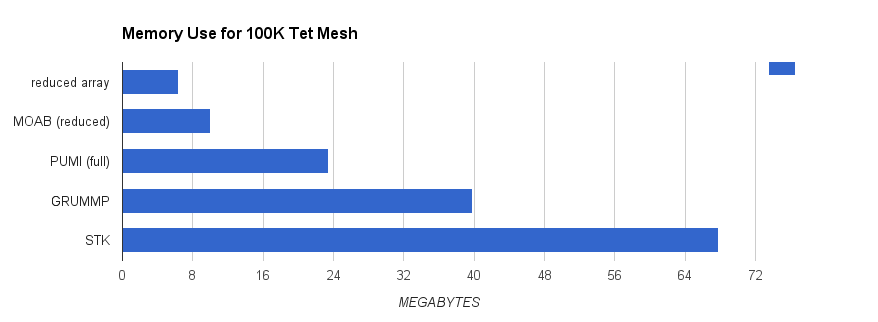
\includegraphics[width=1.0\paperwidth]{notgen/memory_comparison.png}
\end{center}
\end{itemize}
}

\begin{frame}
\frametitle{Test 2: Scalable 1.6B Element Generation} 
\begin{itemize}
\item We start with 100K element mesh on rank 0; repeatedly
refine and re-partition until it is 1.6 billion elements
\item Tests scalability, speed, and memory use
\item Initial mesh and refinement are very uniform
\item Repeat 14 times ($2^{14} = 16384$):
\begin{itemize}
\item use ``Cavity Operator" Edge Splitting to make 2X more elements
(this induces some migration at the boundaries)
\item use global RIB to re-partition to 2X more cores
(this also fixes any load imbalance introduced)
\end{itemize}
\item Whole test is in-memory, no files, one MPI batch job
\end{itemize}
\end{frame}

\begin{frame}
\frametitle{Test 2: Runtime of Steps}
\begin{center}
\includegraphics[width=0.8\textwidth]{scl_time.png}
\end{center}
\begin{itemize}
\item Runtime of the refinement and re-partitioning steps
\item Scales over process count
\end{itemize}
\end{frame}

\begin{frame}
\frametitle{Heap Memory Usage}
\begin{center}
\includegraphics[width=0.8\textwidth]{scl_bal_heap.png}
\end{center}
\begin{itemize}
\item Total program memory measured by Operating System
\item Parts get 200K elements during refinement
(hence max = 2X average)
\item Other components use memory, such as MPI library
\end{itemize}
\end{frame}

\frame{\frametitle{Acknowledgements}
This material is based upon work supported by the
U.S. Department of Energy, Office of Science,
Office of Fusion Energy Sciences and
Office of Advanced Scientific Computing Research under
Award Number DE-SC0006617
(Frameworks, Algorithms, and Scalable Technologies for Mathematics).

\vspace{40pt}

\begin{center}
{\it Thank You... Questions ?}
\end{center}

\vspace{40pt}
}

\end{document}

